\documentclass[a2paper, 12pt]{article}
\usepackage[font={huge, bf}]{caption}
\usepackage{fontspec}
\setmainfont{Arial}
\usepackage{subcaption}
\usepackage{graphicx}
\usepackage{tikz}
\usepackage{tikzsymbols}
\usetikzlibrary{calc,patterns,shapes.geometric}
\usepackage{float}
\usepackage{pdflscape}
\usepackage{geometry}
\geometry{landscape, margin=2cm}
\captionsetup[subfigure]{justification=justified,singlelinecheck=false}
\pagestyle{empty}

\def\centerarc[#1](#2)(#3:#4:#5){\draw[#1] ($(#2)+({#5*cos(#3)},{#5*sin(#3)})$) arc (#3:#4:#5);}

\begin{document}
	\vspace*{\fill}
	\begin{figure}[!htbp]
		\centering
		\begin{subfigure}[b]{0.48\textwidth}
			\caption{Figure 1}
			\centering
			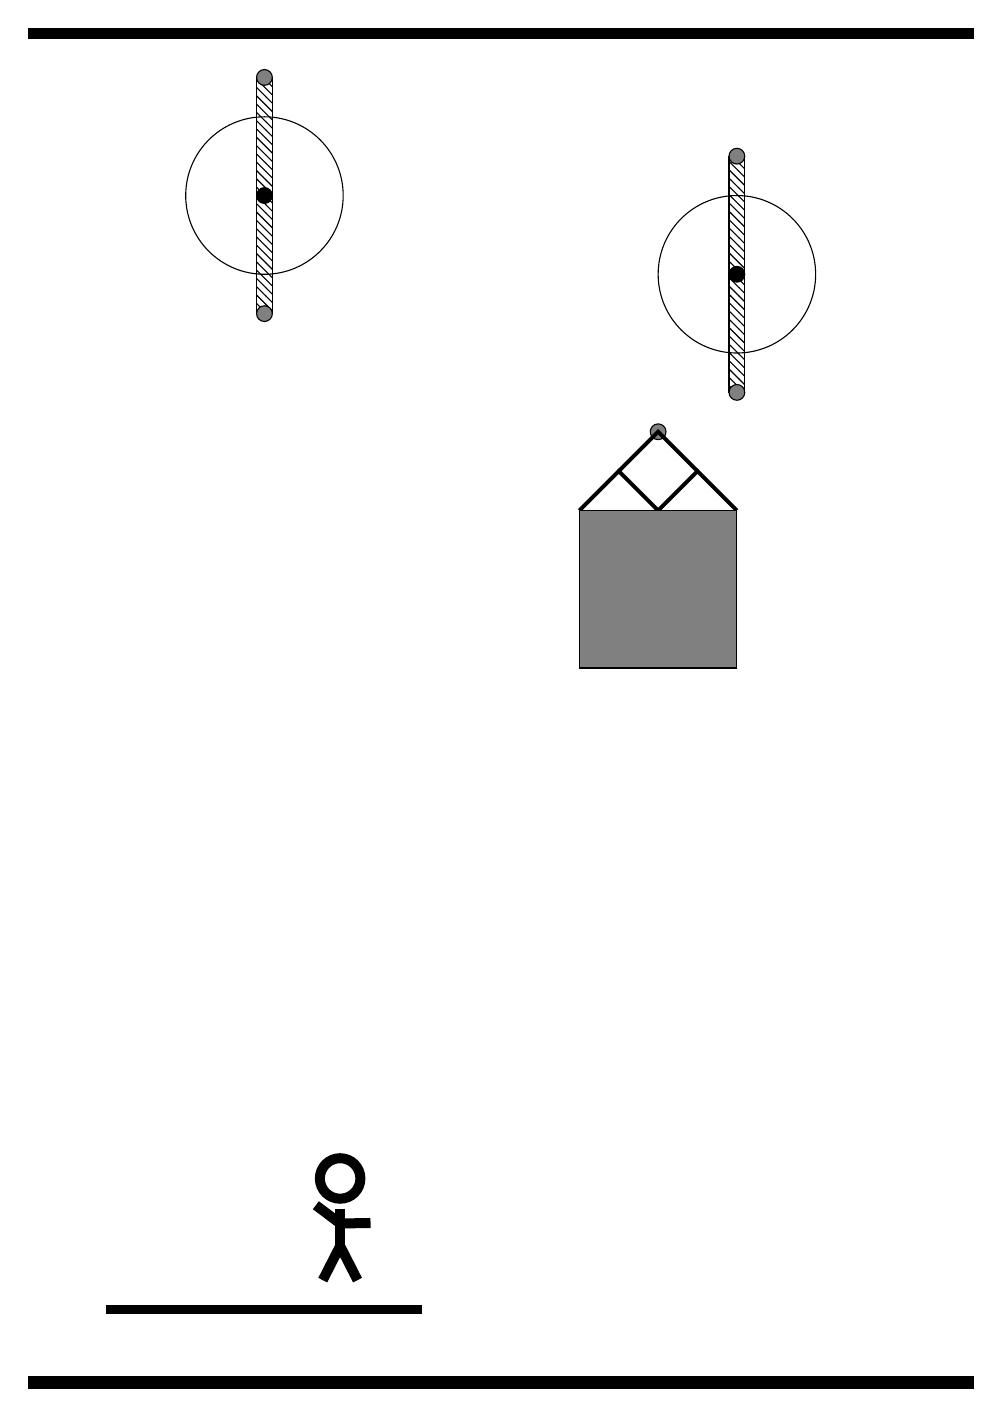
\begin{tikzpicture}
				\draw[fill=black] (-2, 14) rectangle (10, 14.125);
				
				\draw (7,11) circle (1);
				\draw[fill=black] (7,11) circle (0.1);
				\draw[pattern=north west lines, pattern color=black] (6.9,12.5) rectangle (7.1,9.5);
				\draw[fill=black!50] (7,12.5) circle (0.1);
				\draw[fill=black!50] (7,9.5) circle (0.1);
				
				\draw (1,12) circle (1);
				\draw[fill=black] (1,12) circle (0.1);
				\draw[pattern=north west lines, pattern color=black] (0.9,13.5) rectangle (1.1,10.5);
				\draw[fill=black!50] (1,13.5) circle (0.1);
				\draw[fill=black!50] (1,10.5) circle (0.1);
				
				\draw[fill=black!50] (6,9) circle (0.1);
				\draw[line width=0.5mm](5.5,8.5) -- (6,9) --  (6.5,8.5);
				\draw[line width=0.5mm](5,8) --  (5.5,8.5) -- (6,8) -- (6.5,8.5) -- (7,8);
				\draw[fill=black!50] (5, 8) rectangle (7, 6);
				
				\node at (2, -1) {\scriptsize \Strichmaxerl[10][-37][1]};
				\draw[fill=black] (-1, -2.1) rectangle (3, -2.2);
				
				\draw[fill=black] (-2, -3) rectangle (10, -3.15);
			\end{tikzpicture}
		\end{subfigure}
		\hfill
		\begin{subfigure}[b]{0.48\textwidth}
			\caption{Figure 2}
			\centering
			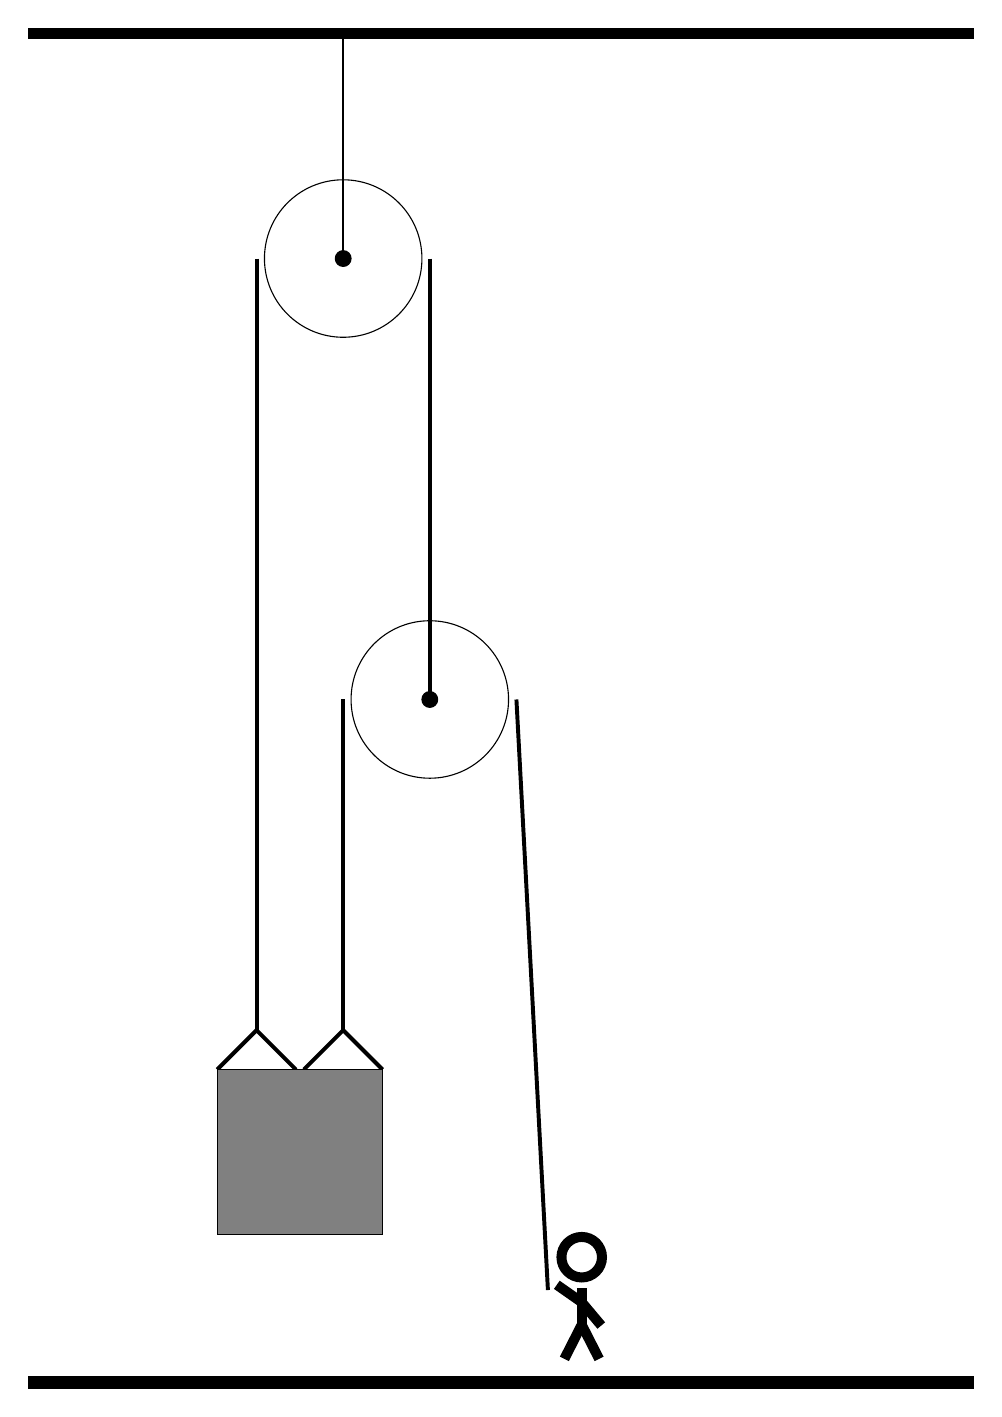
\begin{tikzpicture}
				\draw[fill=black] (-2, 14) rectangle (10, 14.125);
				
				\draw (2, 11.2) circle (1);
				\draw[fill=black] (2, 11.2) circle (0.1);
				\draw[thick] (2, 11.2) -- (2, 14);
				
				\draw (3.1, 5.6) circle (1);
				\draw[fill=black] (3.1, 5.6) circle (0.1);
				
				\draw[line width = 0.5mm]  (0.4, 0.9) -- (0.9, 1.4) -- (1.4, 0.9);
				\draw[line width = 0.5mm]  (1.5, 0.9) -- (2.0, 1.4) -- (2.5, 0.9);
				\draw[fill=black!50] (0.4, 0.9) rectangle (2.5, -1.2);
				
				\draw[line width = 0.5mm] (0.9, 11.2) -- (0.9, 1.4);
				\centerarc[line width = 0.5mm](2, 11.2)(0:180:1.1);
				\draw[line width = 0.5mm] (3.1, 11.2) -- (3.1, 5.6);
				\draw[line width = 0.5mm] (2.0, 5.6) -- (2.0, 1.4);
				\centerarc[line width = 0.5mm](3.1, 5.6)(0:180:1.1);
				\draw[line width = 0.5mm] (4.2, 5.6) -- (4.6, -1.9);
				
				\node at (5, -2) {\scriptsize \Strichmaxerl[10][-35][-50]};
				
				\draw[fill=black] (-2, -3) rectangle (10, -3.15);
			\end{tikzpicture}
		\end{subfigure}
	\end{figure}
		\vspace*{\fill}
\end{document}